\documentclass[journal]{IEEEtran}
\usepackage{graphicx}
\usepackage[spanish]{babel}%\usepackage[utf8]{inputenc}

\begin{document}

\ifCLASSINFOpdf

\else

\fi
% paper title
% can use linebreaks \\ within to get better formatting as desired
\title{Física más allá del modelo estandar}
%

\author{Andrés Arteaga Villarreal~\IEEEmembership{andres.arteaga@udea.edu.co \\ Universidad de Antioquia\\
Facultad de Ciencias Exactas y Naturales.}
         % <-this % stops a space

}

\providecommand{\keywords}[1]{\textbf{\textit{Index terms---}} #1}

\markboth{Instituto de F\'isica, curso de  F\'isica Subatómica, Diciembre~2020}%
{Shell \MakeLowercase{\textit{et al.}}: Bare Demo of IEEEtran.cls for Journals}

\maketitle

\begin{abstract}

\textnormal{
Desde el principio del siglo XX con el surgimiento de nuevas teorías en física como la relatividad y la mecánica cuántica nuevas interpretaciones sobre lo que que constituye el universo han sido desarrolladas. En los años 60 con el descubrimiento de nuevas partículas se propuso un modelo con el cual todas las partículas descubiertas se reducen a solo unas pocas partículas fundamentales con las que se pueden obtener las demás. Esta teoría es el modelo estándar, la cual pretende describir las partículas fundamentales y las interacciones que se dan entre ellas, sin embargo el modelo estándar no ofrece una descripción completa acerca de todo lo que constituye el universo. En este escrito se dará un repaso acerca de los conceptos fundamentales de este modelo teórico y cuales con los actuales desafíos que se presentan para una descripción completa sobre la estructura fundamental del universo.}
\end{abstract}

\begin{keywords}{}
\textnormal{Modelo estándar, materia oscura, energía oscura, supersimetría}
\end{keywords}



\IEEEpeerreviewmaketitle



\section{Introducción}

A finales de siglo XIX el químico ruso Dmitri Mendeleev desarrolló una forma de organizar los componentes que se creían fundamentales y que constituyen la materia, estos son los elementos químicos y con la creación de la tabla periódica se dio uno de los primeros modelos que pretenden organizar los componentes de todo lo que constituye la materia de una manera compacta y precisa. Ver figura~\ref{T Periodica}.

La tabla periódica representó un gran logro en el desarrollo de la química moderna y sobre la manera como se entiende la composición de la materia. Sin embargo, dado que también a finales de este siglo, en 1897 el físico Joseph John Thomson logró identificar experimentalmente al electrón junto con el descubrimiento de otras partículas subatómicas, una nueva concepción sobre la estructura de la materia debía ser desarrollada. 



\begin{figure}[!htb]
  \centering
  \begin{tabular}{@{}c@{}}
    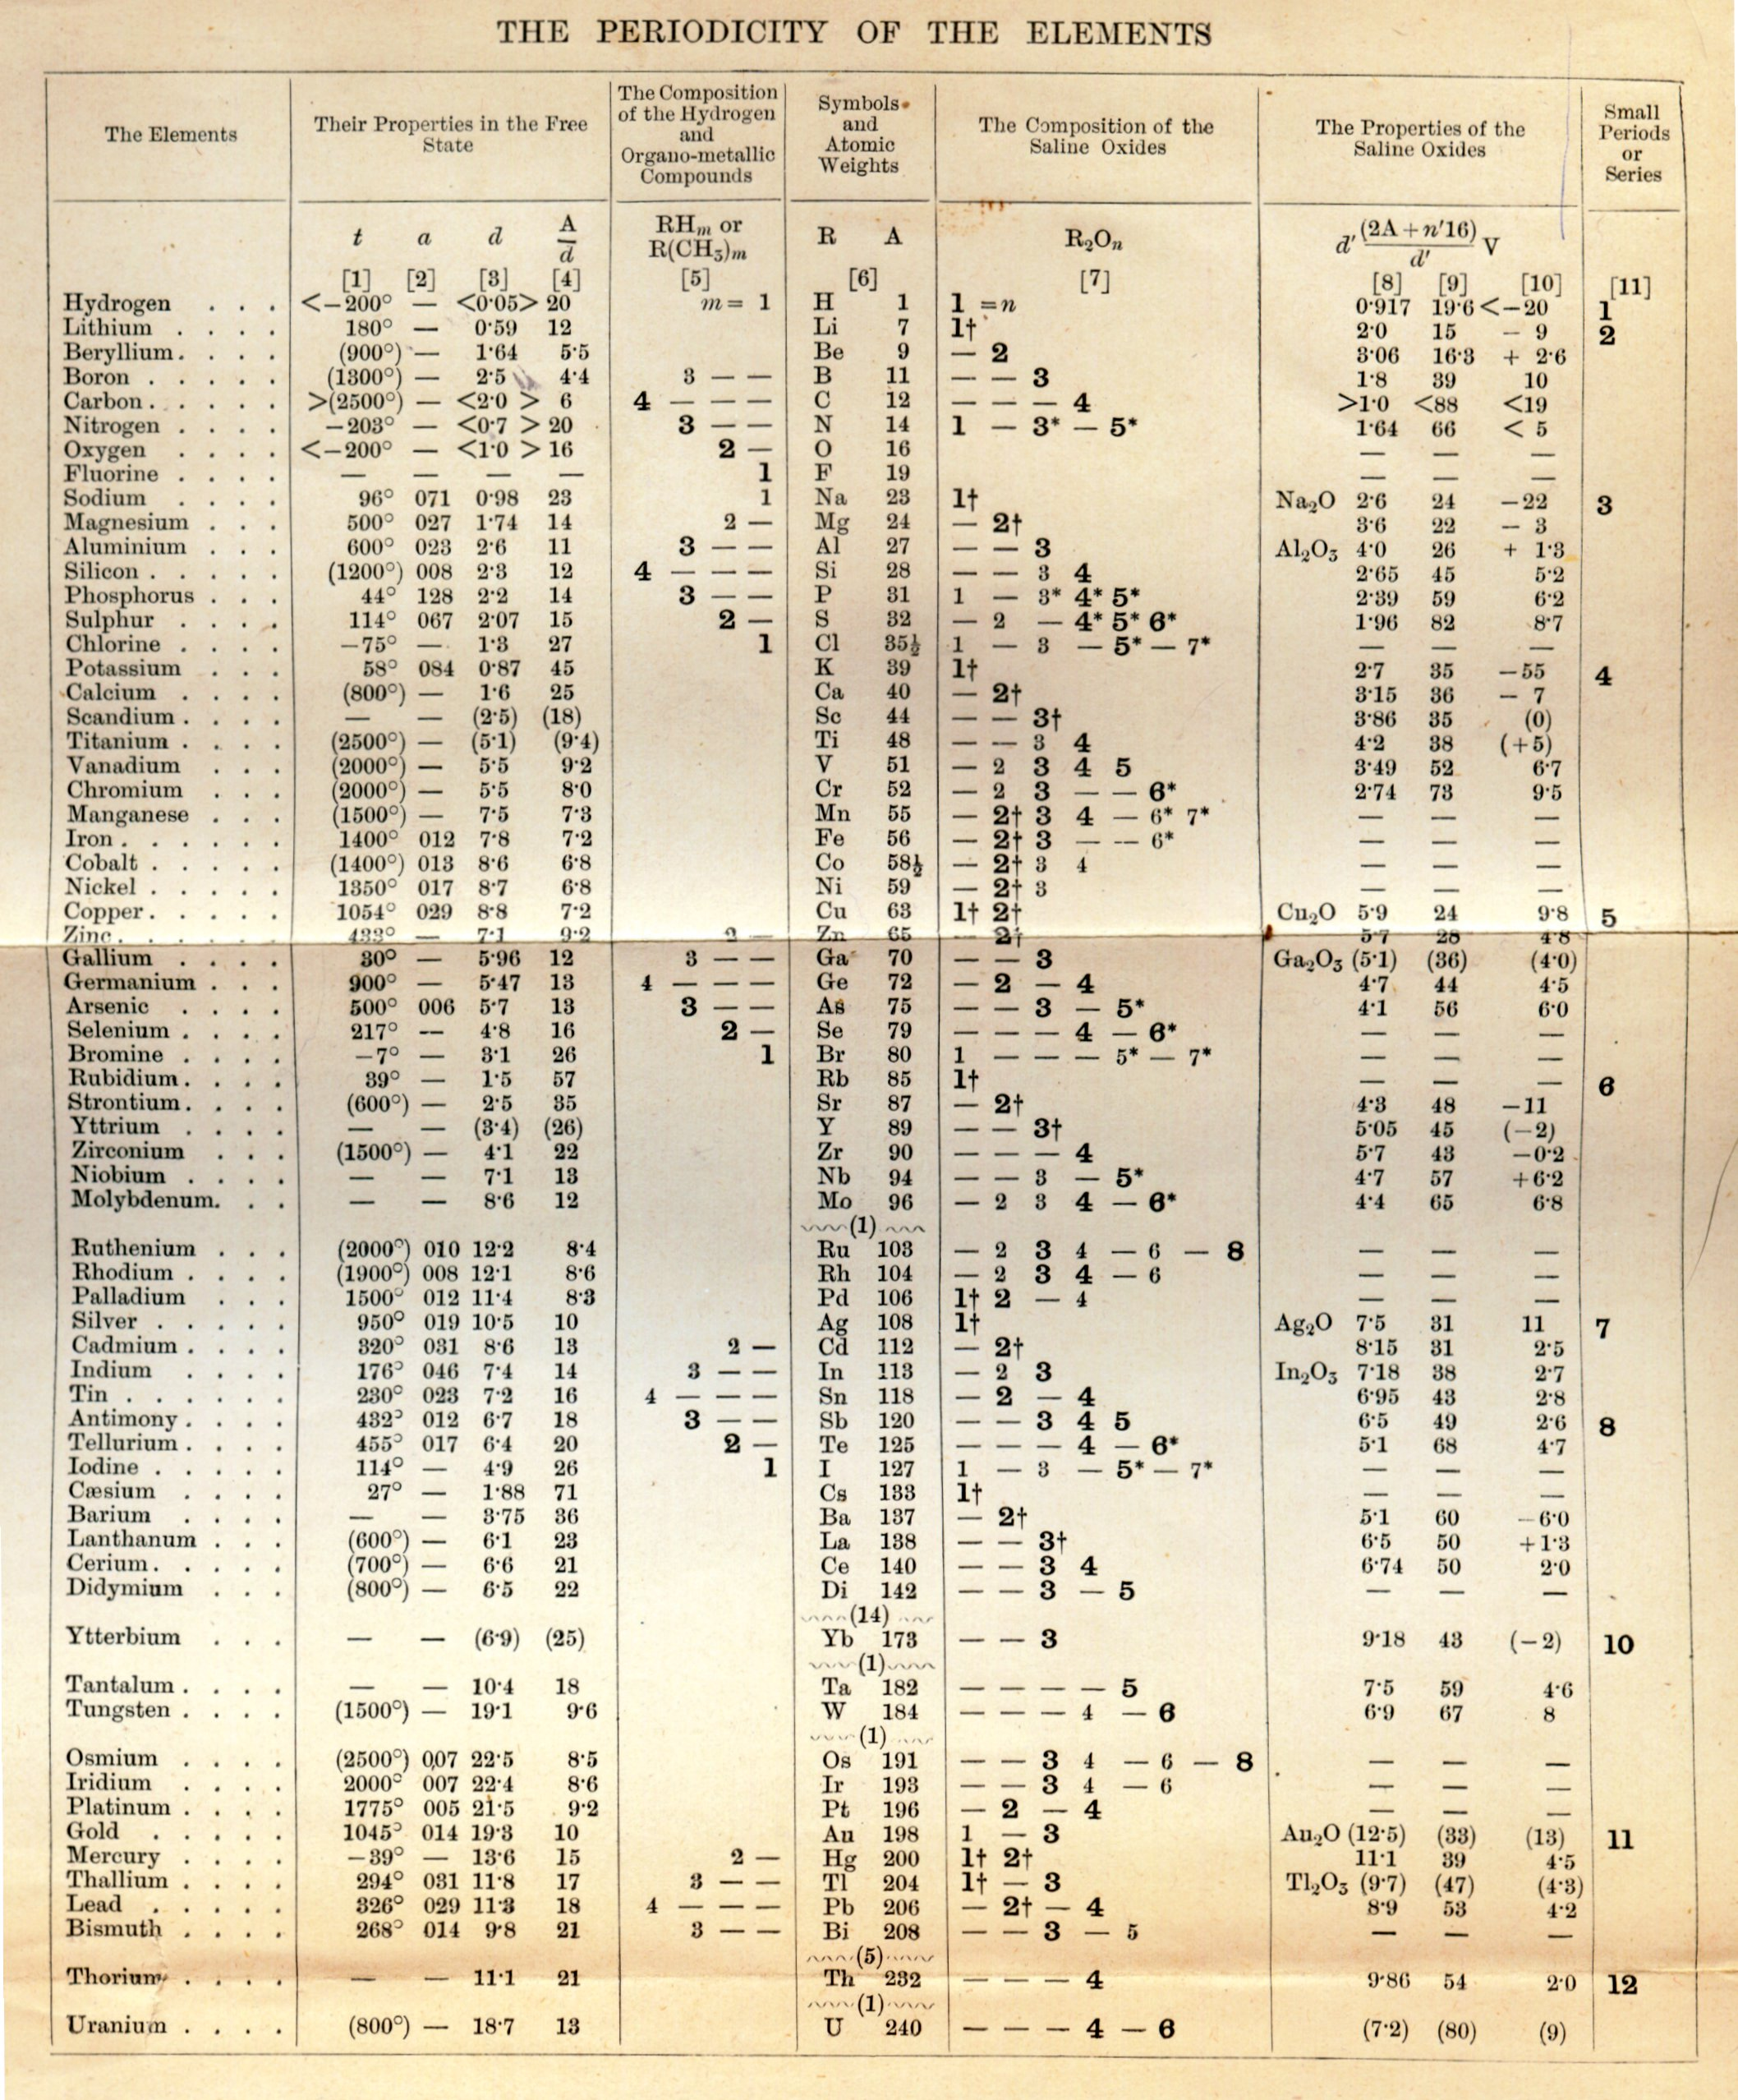
\includegraphics[width=.9\linewidth,height=8 cm
    ]{Mendeleev_Table_5th_II.jpg} \\[\abovecaptionskip]
    \small (a) Tabla periódica desarrollada por Mendeleev (1891).
  \end{tabular}
  \vspace{\floatsep}
  \begin{tabular}{@{}c@{}}
    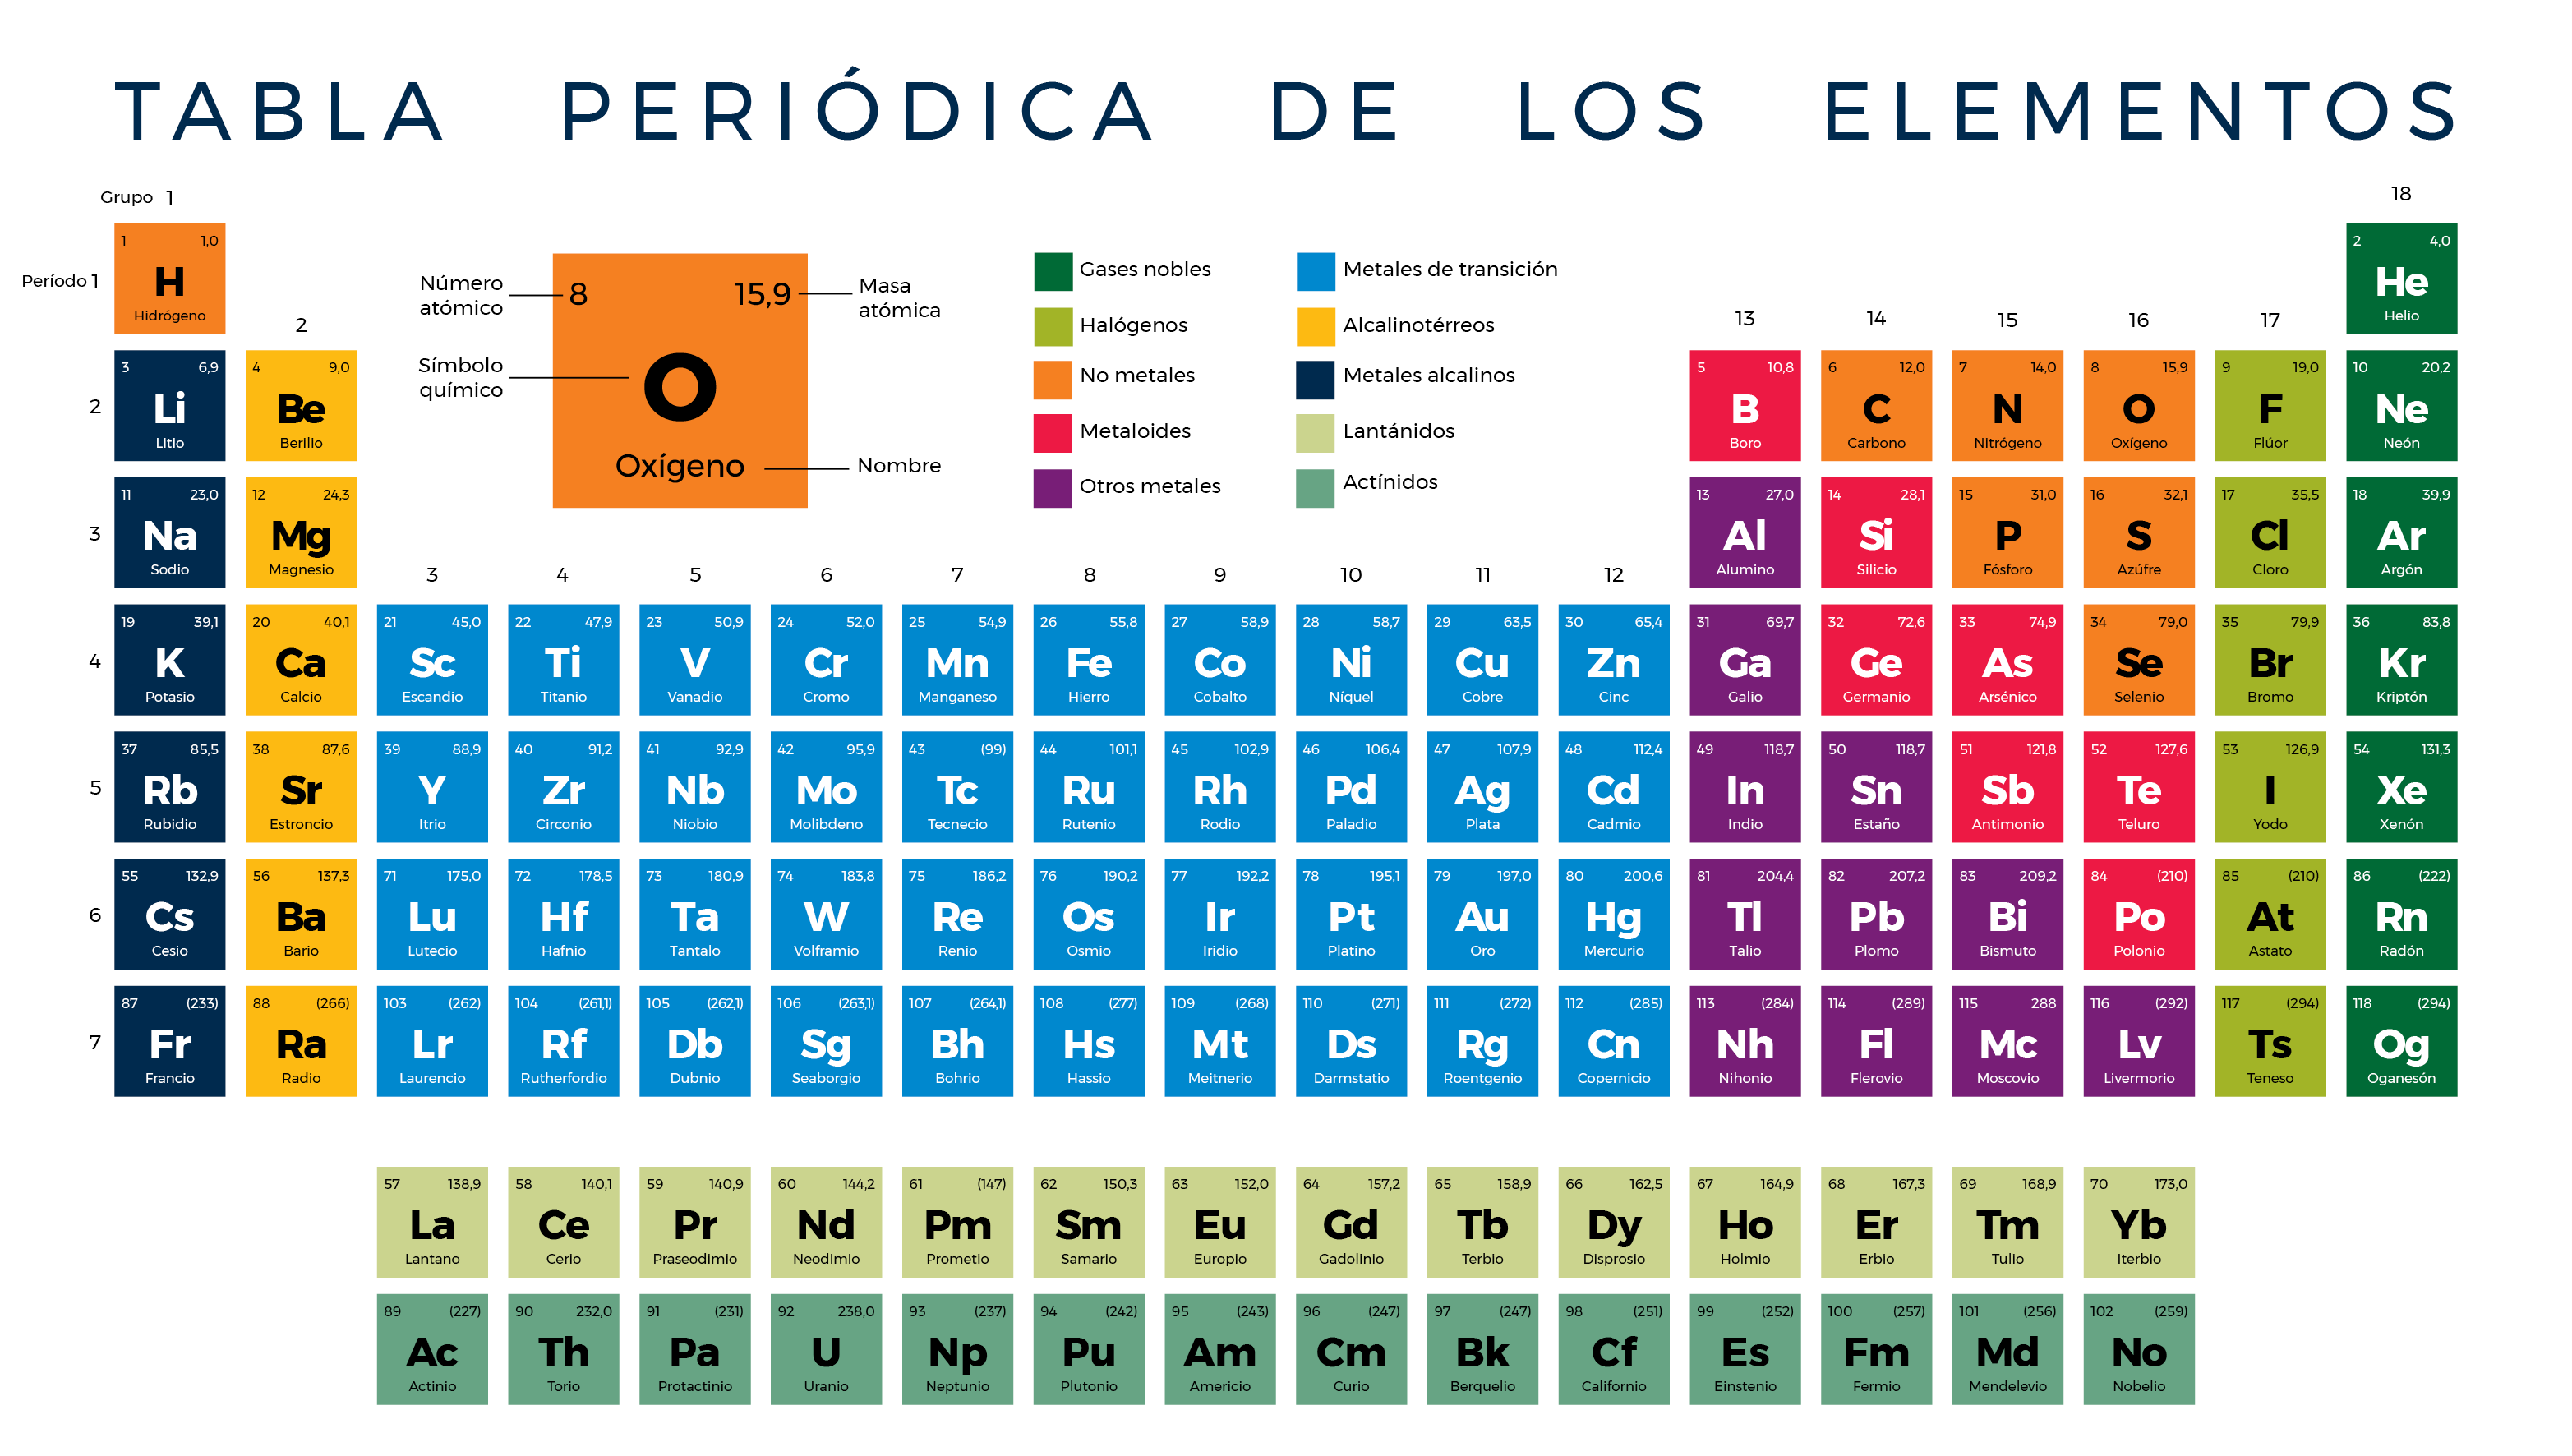
\includegraphics[width=.9\linewidth,height=6cm]{tabla-periodica2.png} \\[\abovecaptionskip]
    \small (b) Tabla periódica actual
  \end{tabular}
  \caption{Evolución de la estructura de la tabla periódica}
\label{T Periodica}
\end{figure}


Después de las grandes revoluciones científicas al principio del siglo XX con la llegada de la mecánica cuántica y la relatividad; ya para el año de 1960 el describir la materia a un nivel puramente atómico apenas daba cuenta de la superficie de lo que es la física de partículas y de todos los fenómenos subatómicos.

Asimismo, para esta época partículas como el muón $\mu^{-}$  y el neutrino electrónico $\nu_{e}$ teorizado por Pauli en 1930 ya habían sido comprobados y detectados experimentalmente, por lo cual una nueva estructura y modelo para tratar con este tipo de partículas debía ser estructurado.


 Con el esfuerzo colectivo de los científicos se desarrolló una nueva imagen sobre la constitución de la materia. Esta imagen redujo todas las partículas conocidas a unas pocas elementales. Y al aplicar un teorema matemático desarrollado por Emmy Noether en 1918 que vincula las simetrías con las leyes de conservación de la naturaleza al mundo subatómico, se colocó estas partículas fundamentales en listas y grupos, muy parecido a la tabla periódica de elementos. Esto ayudó a los físicos de partículas a buscar patrones y vínculos. A mediados de la década de 1970, la teoría estaba tan bien establecida que se conoció como Modelo Estándar~\cite{IOP}
 
 
 Esta nueva concepción sobre la naturaleza fundamental de la materia hizo de la tabla periódica un modelo complementario el cual daba cuenta del entendimiento de la química de los elementos presentes en el universo, mas no un modelo que describe la composición de la materia a un nivel fundamental.
 
 \section{El modelo estándar}
 
 
 
\begin{figure}[!htb]
\centering
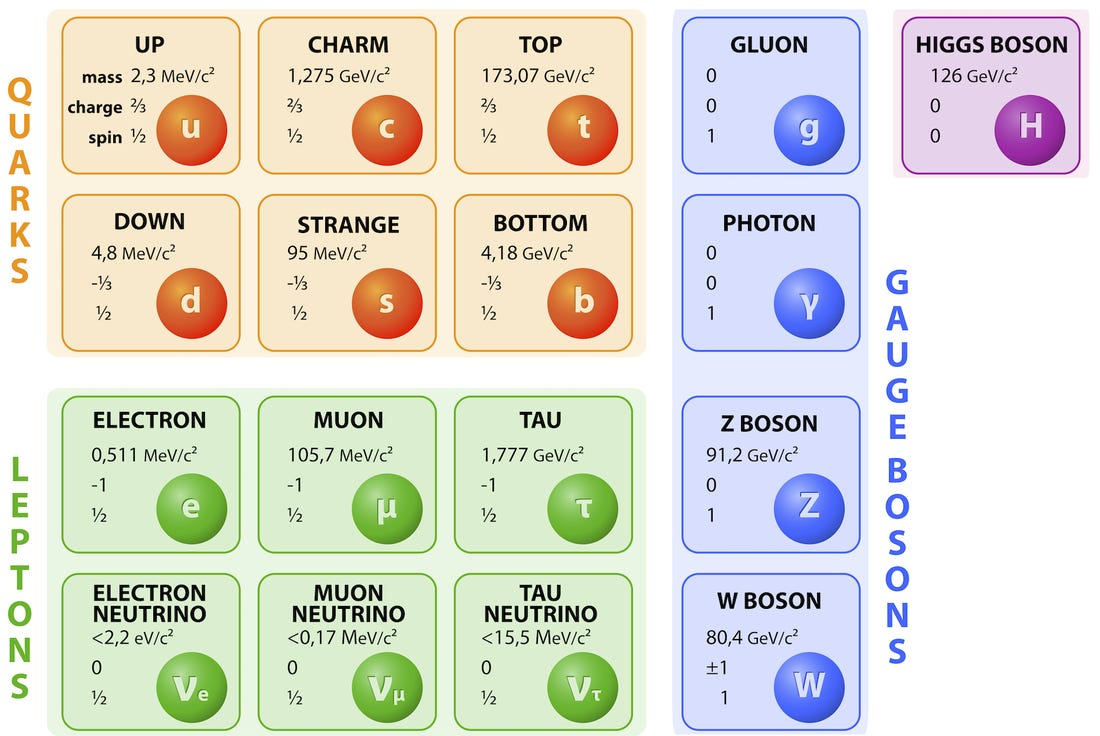
\includegraphics[width=\linewidth,height=8 cm]{ModeloEstandar.png}
\caption{ Estructura de modelo estándar en la actualidad}
\label{Modelo Estandar}
\end{figure}

El modelo estándar (SM) es una teoría cuántica de campos basada en los grupos gauges de color SU(3), quiral SU(2) y U(1) que están asociados con la cromo-dinámica cuántica (QCD), las interacciones débiles y la electrodinámica cuántica (QED)~\cite{S.D. Bass}. El modelo estándar permite entender como estas partículas fundamentales interactúan entre si y como estas forman nuevas partículas.

Las interacciones que se pueden explicar a través del SM son: \emph{la interacción débil}, la cual es responsable del decaimiento radioactivo, el ejemplo más conocido es el decaimiento beta de los neutrones en el núcleo atómico.

La segunda interacción fundamental es \emph{la interacción fuerte}, que es la que se encarga de mantener unido el núcleo atómico que se conforma de protones y neutrones, esta interacción evita que los protones dentro del núcleo se separen debido a su carga eléctrica, pues según la ley de Coulomb las cargas iguales se repelen.

La tercera interacción fundamental es \emph{la interacción electromagnética}, que como su nombre indica describe los fenómenos eléctricos, magnéticos y la radiación.  

El modelo estándar consta hasta ahora de 17 partículas fundamentales (ver figura \ref{Modelo Estandar}). 12 de ellas son \emph{fermiones}, que son los componentes básicos de la materia; los ferminoes se dividen en 6 \emph{quraks} estos son: up, down, top, bottom, charm y strange y  6 \emph{leptones} que son: electrón $e^{-}$, muon $\mu^{-}$, tau $\tau^{-}$, neutrino electrónico $\nu_{e}$, neutrino muónico $\nu_{\mu}$ y neutrino tau $\nu_{\tau}$.

Las 5 partículas restantes son los llamados \emph{bosones}, responsables por la interacción entre la  materia, estos son: el fotón $\gamma$, asociado a la interacción electromagnética, los bosones $Z$ y $W$, se encargan de la interacción debil, el gluón $g$ responsable de la interacción fuerte y el bosón de Higgs $H$ el cual se encarga de dar masa a las partículas fundamentales.

El modelo estándar también tiene en cuenta las diferentes simetrías y por lo tanto se tienen cantidades asociadas que se conservan, como lo es la conservación de la carga, del momento, del número leptónico, entre otros.

El modelo estándar explica lo concerniente a toda la materia que podemos observar en el día a día, sin embargo esta materia, llamada materia bariónica, solo constituye el 5\% de todo lo que está presente en el cosmos, el 95\% restante se divide entre \emph{materia oscura}, la cual constituye al rededor de un 26\% del universo y el 69\% restante es la llamada \emph{energía oscura}.

 \section{Materia oscura y energía oscura}

\subsection{Materia oscura}

Las primeras evidencias experimentales sobre la denominada materia oscura (DM) por sus siglas en inglés, fueron obtenidas a través del trabajo de los astrónomos y su estudio sobre la velocidad de las estrellas dentro de una galaxia.
A principios de la década de 1930, Oort descubrió que el movimiento de las estrellas en la Vía Láctea insinuó la presencia de mucha más  masa galáctica de lo que nadie había predicho anteriormente~\cite{K. Garrett}.

Se asumía que las estrellas dentro de una galaxia tendrían un comportamiento muy similar al de los planetas en el sistema solar, por lo que se esperaba que la velocidad fuera de la forma $ v(r) = \sqrt{G\frac{m(r)}{r}}$, con $G$ la constate de gravitación y $m(r)$ la masa contenida dentro de un radio $r$. 

De esta ecuación se entiende que la velocidad es inversamente proporcional a la distancia de su centro, lo que se conoce como comportamiento Kepleriano, sin embargo, los resultados experimentales arrojaron resultados completamente diferentes, observándose que la velocidad de las estrellas no disminuye a medida que se alejan del centro sino, al contrario, esta aumenta hasta después alcanzar un valor límite. Ver figura \ref{Velocidades}.


\begin{figure}[!htb]
\centering
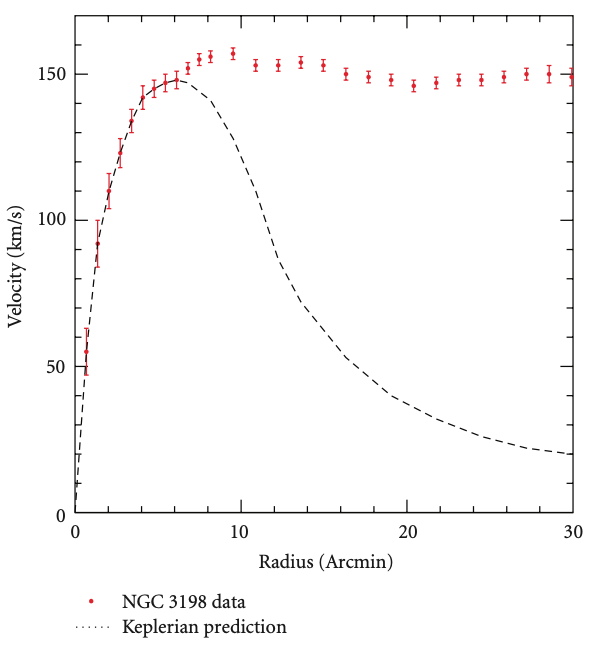
\includegraphics[width=\linewidth,height=8 cm]{velociad.png}
\caption{ Medidas de las velocidades rotacionales en regiones HI  en  NGC 3198 comparado con el idealizado comportamiento Kepleriano. Tomado de \hspace{.2cm}\cite{K.G. Begeman}.}
\label{Velocidades}
\end{figure}

La masa presente dentro de las galaxias interactúa con la luz, ya sea reflejándola, absorbiéndola o emitiéndola, es a través de este tipo de interacciones que se puede estimar la masa de una galaxia, si se calcula la la velocidad rotacional de una galaxia utilizando solo la materia que interactúa con la radicación, se encuentran resultados que no concuerdan con los datos experimentales, es por esto que se deduce la presencia de algún tipo de materia extra la cual no podemos observar.

Este tipo nuevo de materia es la llamada materia oscura, se denomina oscura debido a que este tipo de materia no se ve afectada por la interacción electromagnética. Además ninguna de las partículas del modelo estándar serían candidatas para la generación de dicho tipo de materia, pues, la materia oscura es afectada por la interacción gravitacional, y esta interacción es precisamente la que no se tiene en cuenta y no puede ser descrita por el modelo estándar.

\subsection{Energía oscura}

Ya desde principios de la década de los 90 se conocía que el universo se estaba expandiendo, sin embargo, se pensaba que esta expansión iba desacelerando a medida que trascurría el tiempo, esto debido a que la masa presente en el universo interactuaría entre si por medio de la gravedad y esto haría que el universo desacelere en su expansión y eventualmente este volvería comprimirse debido a efectos gravitacionales.

 El telescopio espacial Hubble (HST) descubrió que la radicación proveniente de galaxias lejanas sufría un corregimiento al rojo \emph{'red shift'}. La longitud de onda de la radiación proveniente de estas galaxias se hace cada vez más grande a medida que estas se alejan unas de otras causando el red shift. 
 
 Lo anterior era consistente con la idea de un universo en expansión, sin embargo, en 1998 con el estudio independiente de dos proyectos, el \emph{Supernova Cosmology Project} y el \emph{High-z Supernova Search Team} donde con el estudio de supernovas tipo A, se obtuvo la increíble conclusión de que el universo no solo se está expandiendo sino que lo hace cada vez más rápido a medida que transcurre el tiempo.

Aceptando la validez de la relatividad general, teoría que describe la interacción gravitacional, esta expansión solo puede ser explicada por la presencia de una energía que no proviene de las masas de la materia común, sino que es un tipo de energía intrínseca al espacio vació, este nuevo tipo de energía fue denominada por los científicos como energía oscura (DE) por sus siglas en ingles. La energía oscura sigue siendo un misterio para la física actual y uno de los más grandes desafíos para la comprensión del universo..

Una posible solución  a la explicación de la energía oscura es la constante cosmológica, que a diferencia de como Einstein la propuso inicialmente en 1917 para un modelo estático del universo, esta constante puede en cambio ser utilizada para explicar la expansión acelerada del cosmos. Actualmente aun no se tiene claridad respecto a la naturaleza de la energía oscura y la única evidencia de su existencia son sus efectos en la ya comprobada expansión del universo. Ver figura 4.

\begin{figure}[!htb]
\centering
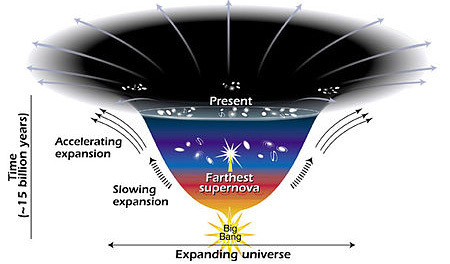
\includegraphics[width=.9\linewidth,height=6 cm]{DarkEnergy.jpg}
\caption{Diagrama que  muestra los cambios en la expansión del universo desde su nacimiento aproximadamente hace 15 mil millones de años, entre mas plana es la curva mas rápido se expande el universo. Tomada de \hspace{.2cm}\cite{Nasa}}
\label{Dark Energy}
\end{figure}

\section{Supersimetría}

Para entender el concepto de supersimetría primero se debe entender la necesidad de dicho concepto, lo que se conoce como el problema de la jerarquía.

El problema de la jerarquía surge de la predicción del SM del valor esperado del vacío de Higgs (es decir, el valor promedio del campo en el vacío), que es de aproximadamente 246 GeV. Los teóricos han predicho que a energías suficientemente altas ($\approx$1 TeV) las fuerzas electromagnéticas y débiles actúan como una sola fuerza unificada llamada fuerza electrodébil (esto también se ha verificado experimentalmente). Sin embargo, a energías más pequeñas, la única fuerza unificada se descompone en dos fuerzas separadas: la fuerza electromagnética y la fuerza débil. Resulta que después de esta ruptura, el estado de energía más bajo del campo de Higgs no es cero, sino el valor esperado de vacío de 246 GeV. Es precisamente este valor distinto de cero el que da masa a otras partículas a través de sus interacciones con el campo de Higgs. El valor de 246 GeV está en la escala débil (la energía típica de los procesos electrodébiles); sin embargo, en la escala de Planck (la energía a la que los efectos cuánticos de la gravedad se vuelven fuertes) es de alrededor de $10^{19}$ GeV. La pregunta básica, entonces, es ¿por qué la escala de Planck es $10^{16}$ veces mayor que la escala débil? ¿Existe simplemente un ``desierto'' entre $10^{3}$ y $10^{19}$ GeV en el que no entra ninguna nueva física? \cite{K. Garrett}.

Se podría suponer por un momento que el SM  puede describir de manera correcta los fenómenos físicos hasta el orden de magnitud de la escala de Plank. En ese caso la masa del bosón de Higgs debería de ser del mismo orden, es decir de $10^{16}$ TeV, sin embargo, si la masa del Higgs es superior a 1 TeV aparecen inconsistencias en el Modelo Estándar.\hspace{.2cm}\cite{P. Gonzales}

Ante estas inconsistencias en el modelo estándar surge el modelo de supersimetría (SUSY, ver figura \ref{SUSY}), este modelo es una extensión del modelo estándar tradicional y dúplica la cantidad de partículas del modelo original añadiendo a cada partícula una compañera. Esta compañera tendrá las mismas propiedades que su análogo en el modelo original salvo por una, el spin. Esta nueva simetría sobre el spin hace que se puedan hacer un nuevo tipo de operación sobre la partícula tal que cambie el valor del spin, pero deja el resto de propiedades (masa y carga) iguales.

Las compañeras del modelo SUSY para los ferminoes se denominan con nombres que comienzan con 's', así la compañera supersimétrica del electrón es el selectrón, la del muon es smuon; y para los bosones, las compañeras supersimétricas reciben nombres que terminan en 'ino', así la compañera supersimétrica del fotón es el fotino.

\begin{figure}[!htb]
\centering
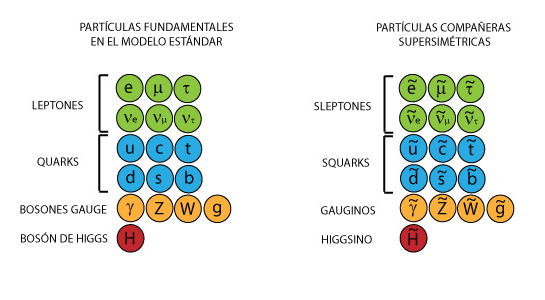
\includegraphics[width=\linewidth,height=6 cm]{Supersimetria.jpg}
\caption{Diagrama que  muestra las partículas originales del SM y la extensión de supersimetría donde a cada partícula se le asigna un compañera supersimétirca}
\label{SUSY}
\end{figure}


En principio el modelo SUSY podría a simple vista resultar menos atractivo para un modelo que contenga los bloques fundamentales que constituyen la realidad, puesto que en un principio no se necesitan ninguna de estas partículas adicionales para describir una interacción fundamental. Sin embargo, utilizando SUSY es posible resolver el problema de la jerarquía, además de brindar una posible explicación a la existencia de la materia oscura.

A pesar de todas estas posibles soluciones a los problemas que presenta el modelo estándar, la presencia de la supersimetría en la naturaleza aun no se comprobado experimentalmente haciendo del modelo SUSY aun un modelo puramente teórico. 



\section{conclusión}

El modelo estándar representa uno de los logros más significativos de la física teórica actual, con la reciente comprobación experimental del bosón de Higgs en el LHC en 2012, el modelo estándar tiene un sustento teórico y experimental lo suficientemente completo y preciso para describir 3 de las 4 interacciones fundamentales, sin embargo, el modelo aun no es capaz de resolver todos los problemas que surgen cuando se empieza a trabajar en escalas de altas energías donde los efectos de la gravedad deben ser tenidos en cuenta.

Si bien los efectos gravitacionales no son apreciables a una escala subatómica, si se deben tener en cuenta para describir procesos cosmológicos como los que involucran el origen del universo y es por esto que se debe dar un desarrollo más a fondo del modelo estándar ya sea el de supersimetría SUSY o algún otro el cual permita tener una descripción mas general y unificada sobre las 4 interacciones fundamentales, este modelo claro está debe también ser consistente verificable de manera experimental.





\begin{thebibliography}{1}

\bibitem{IOP}
Institute of Physics (IOP), \emph{The Standard Model}, en linea: https://www.iop.org/explore-physics/physics-stepping-stones/standard-model. Consultado en diciembre 2020

\bibitem{S.D. Bass}
S. D. Bass, \emph{Emergent gauge symmetries and particle physics}\\ DOI:\emph{ 10.1016/j.ppnp.2020.103756}

\bibitem{K. Garrett}
K. Garrett \& G. Duda \emph{Dark Matter: A Primer}\\
DOI:\emph{10.1155/2011/968283}

\bibitem{K.G. Begeman}
K. G. Begeman \emph{H I rotation curves of spiral galaxies}, Astronomy and Astrophysics, vol. 223, pp. 47–60, 1989.

\bibitem{Nasa}
NASA \emph{Dark Energy, Dark Matter}, en linea: https://science.nasa.gov/astrophysics/focus-areas/what-is-dark-energy.
Consultado en diciembre 2020

\bibitem{P. Gonzales}
P. González \& F. Marchesano \emph{Jerarquía y Supersimetría}, Ivestigación y Ciencia, en linea: https://www.investigacionyciencia.es/blogs/fisica-y-quimica/29/posts/jerarqua-y-supersimetra-10446.
Consultado en diciembre 2020


\end{thebibliography}




\end{document}


